\chapter{Figures}
\label{ch:figures}

% h means here: Place the figure in the text where the figure environment is written, if there is enough room left on the page
% t means top: Place it at the top of a page.
% b means bottom: Place it at the bottom of a page.
% p means page: Place it on a page containing only floats, such as figures and tables.

% ! allows to ignore certain parameters of LaTeX for float placement (think of it as forcing a parameter)

\begin{figure}[!h]  
    \centering
    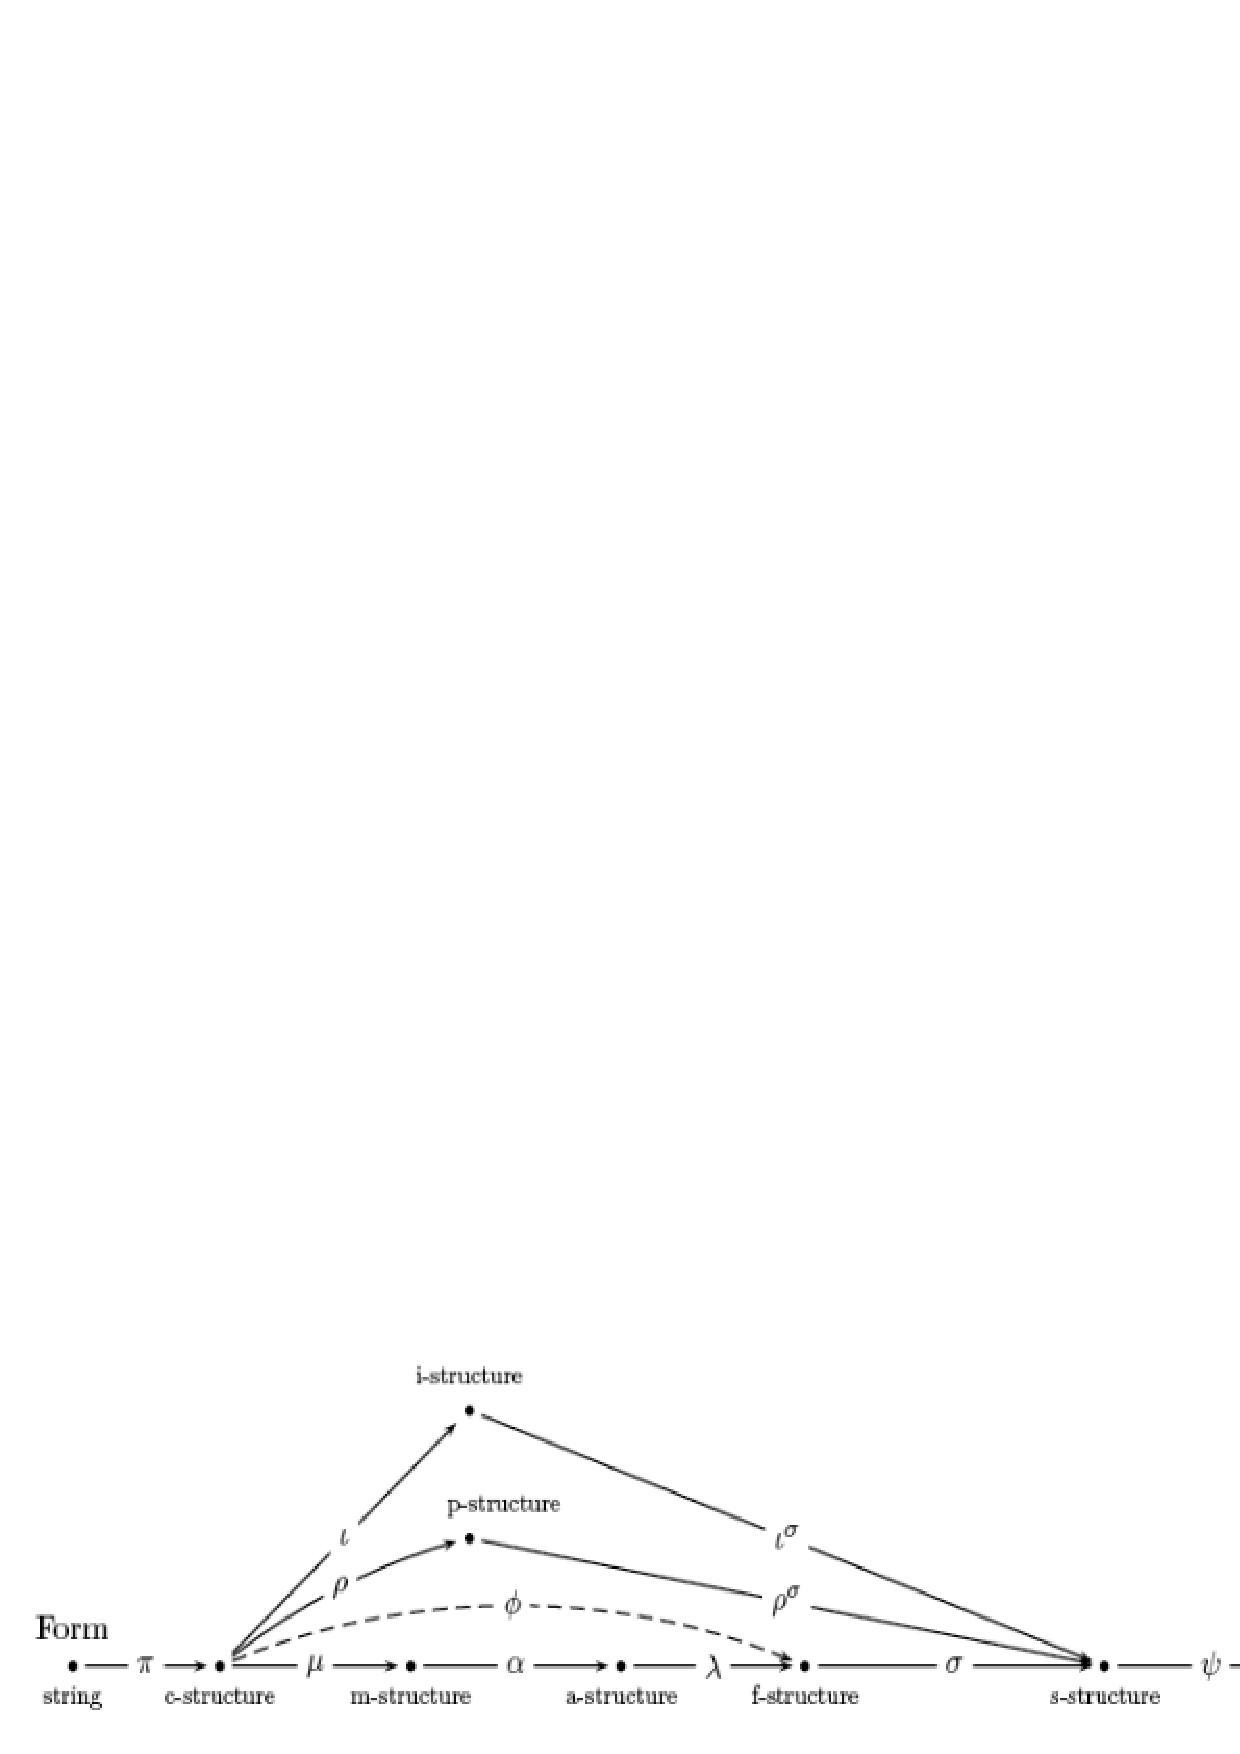
\includegraphics[scale=0.5]{upload/tex/figures/parallelprojection.png}
    \caption{This is the projection architecture}
    \label{fig-label1}
\end{figure}

\begin{figure}[!b]  
    \centering
    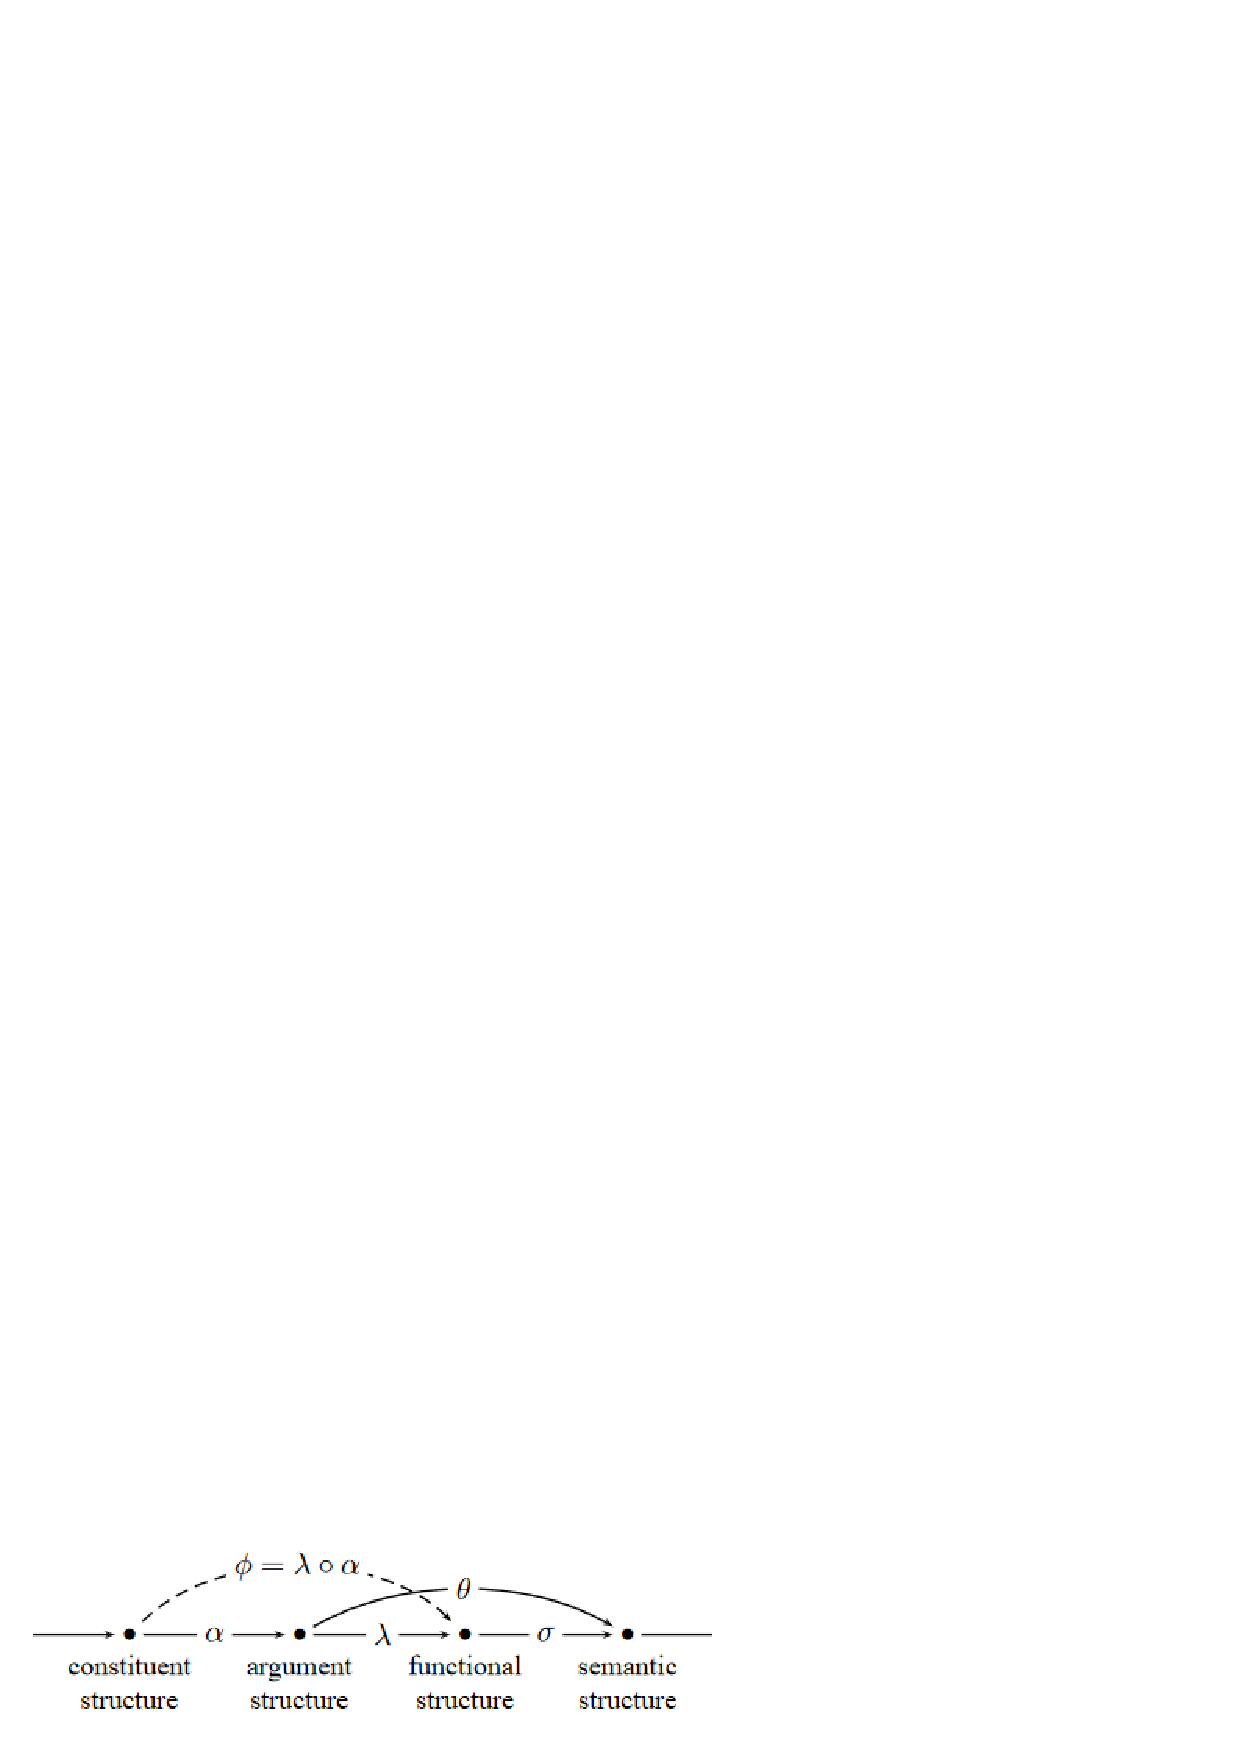
\includegraphics[width=.9\textwidth]{upload/tex/figures/mapping-functions.png}
    \caption{Mapping functions}
    \label{fig-label1}
\end{figure}

\begin{figure}[!t]  
    \centering
    \includegraphics[height=1cm]{upload/tex/figures/UniKonstanz-Logo-Optimum-sRGB.jpg}
    \caption{Uni Konstanz Logo}
    \label{fig-label1}
\end{figure}